%====================================================================================
\section{Motivation}
%====================================================================================

\begin{frame}{Unobserved-Heterogeneity}
	\begin{itemize}
		\item Controlling unobserved time invariant heterogeneity in cross-sectional models.	
		\item Dynamics of cross-sectional populations through time; change in permanent component of each household or unit across time.
	\end{itemize}
\end{frame}
%------------------------------------------------
\begin{frame}{Unobserved-Heterogeneity}
	\textbf{Identification problem}. Considering the following
		\begin{align*}
			\text{true model} \quad :& \quad Y=X_{1}\beta _{1}^{\ast }+X_{2}\beta_{2}+u \\
			\text{estimated model} \quad :& \quad Y=X_{1}\beta _{1}+u
		\end{align*}
	having the classical properties e.g $u$ is $i.i.d$. we estimate the model%
		\begin{align}
			\widehat{\beta }_{1} = &\left( X_{1}^{\prime }X_{1}\right)^{-1}X_{1}^{\prime }Y  \notag \\
			\widehat{\beta }_{1} = &\left( X_{1}^{\prime }X_{1}\right)
			^{-1}X_{1}^{\prime }\left( X_{1}\beta _{1}^{\ast }+X_{2}\beta _{2}+u\right) 
			\notag \\
			\widehat{\beta}_{1} = &\beta_{1}^{\ast}+\left(X_{1}^{\prime}X_{1}\right)^{-1}X_{1}^{\prime}X_{2}\beta_{2}+\left(X_{1}^{\prime}X_{1}\right) ^{-1}X_{1}^{\prime}u
		\end{align}
	the estimator is biased.
\end{frame}
%------------------------------------------------
\begin{frame}{Unobserved-Heterogeneity}
		\begin{align}
			E\left( \widehat{\beta }_{1}\right) = &\beta _{1}^{\ast }+\left(X_{1}^{\prime }X_{1}\right) ^{-1}X_{1}^{\prime }X_{2}\beta _{2}  \notag \\
			E\left( \widehat{\beta }_{1}\right) = &\beta _{1}^{\ast }+\frac{cov\left(X_{1},X_{2}\right) }{var\left( X_{1}\right) }\beta _{2}
		\end{align}
	We have effects in the variance as well%
		\begin{gather}
			var\left( \widehat{\beta }_{1}\right) -var\left( \widehat{\beta }_{1}^{\ast}\right) =\sigma ^{-2}\left( \left( X_{1}^{\prime }X_{2}\right) \left(X_{1}^{\prime }X_{2}\right) ^{-1}\left( X_{1}^{\prime }X_{2}\right) \right)
		\end{gather}
	above expression is positive
\end{frame}
%------------------------------------------------
\begin{frame}{Unobserved-Heterogeneity}	
	why is this important?
		\begin{figure}
			\centering
				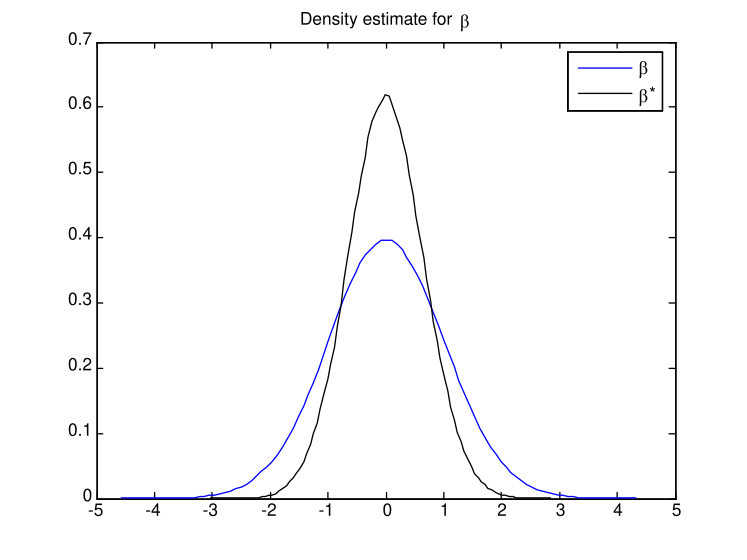
\includegraphics[width = 0.6\linewidth]{figures/density.png}
		\end{figure}
\end{frame}
%------------------------------------------------
\begin{frame}{Unobserved-Heterogeneity}
	\textbf{Identification problem}. What if we have redundant variables?.Considering the following
		\begin{align*}
			\text{estimated model}\quad :& \quad Y=X_{1}\beta_{1}+X_{2}\beta_{2}+u \\
			\text{true model}\quad :& \quad Y=X_{1}\beta_{1}^{\ast}+u
		\end{align*}
	having the classical properties e.g $u$ is \emph{i.i.d}. In this particular case $X_{1}=\iota_{T}$ (the true model just has a constant). We estimate the model with the classical procedure of deviations from time means:
		\begin{align}
			\widehat{\beta}_{2} & = \left(\widetilde{X}_{2}^{\prime}\widetilde{X}_{2}\right)^{-1}\widetilde{X}_{2}^{\prime}\widetilde{Y} \notag \\
			\widehat{\beta}_{2} & = \left(\widetilde{X}_{2}^{\prime}\widetilde{X}_{2}\right)^{-1}\widetilde{X}_{2}^{\prime}\left(\widetilde{X}_{1}\beta_{1}^{\ast}+\widetilde{u}\right) \notag \\
			\widehat{\beta}_{2} & = 0
		\end{align}
	getting the constant $\beta_{1}^{\ast }=\overline{Y}-\overline{X}_{2}\widehat{\beta}_{2}=\overline{Y}$
\end{frame}
%------------------------------------------------
\begin{frame}{Unobserved-Heterogeneity motivation}
	If we have redundant variables in our regression model
		\begin{itemize}
			\item OLS estimator is unbiased and consistent
		\end{itemize}
\end{frame}
%------------------------------------------------
\begin{frame}{Observables and Unobservables}
	In some cases we would expect correlation between unobservales and observables. For instance in the demand- and supply-equation model
		\begin{align}
			Q^{d} & = p^{\prime }\beta +\left( f^{\prime }\gamma +\epsilon \right) \label{demand equation} \\
			p     & = Q^{s\prime}\phi +\psi  \notag
		\end{align}
	being $\beta <0$ and $\phi >0.$ $f$ is an unobservable variable (shocks related to preferences, culture) In equilibrium:
			$$p=\frac{f^{\prime }\gamma \phi }{\left( 1-\beta \right) }+\frac{\epsilon \phi +\psi }{\left( 1-\beta \right)}$$
	So, $E\left( p,f\right) \not=0.$ In a regression model, we wonder if we have a demand or supply equation.
\end{frame}
%------------------------------------------------
\begin{frame}{Observables and Unobservables}
	\begin{itemize}
		\item Classical approach to pinpoint demand equation is to regress quantity on price, because of correlation between price and unobservable the classical strategy is useless.
		\item Strategies for identifying demand equation is available in econometric literature (see Gujarati). For example we suppose that supply equation is given by:
				$$p=\rho p_{-1}+Q^{s\prime }\lambda +\xi$$
		so a valid instrument should be $Z=p_{-1}$, thus the staregy of identification would be%
				$$Q^{d}=Z^{\prime }\beta +\zeta$$
		because of $E\left( Z,f\right) =0.$
	\end{itemize}
\end{frame}
%------------------------------------------------
\begin{frame}{Observables and Unobservables}
	\begin{itemize}
		\item Earnings equations:
					$$wage_{it}=\alpha +\alpha _{s}\cdot schooling_{it}+\alpha_{u}Union_{it}+\varepsilon _{it}$$
			  thus estimator of $\alpha ^{\prime }s$ is $E\left( X_{it}\prime \varepsilon_{it}\right) =0.$ But, ability is correlated with schooling, so makes sense to have a model including a individual specific variable or endownment
					$$wage_{it}=\alpha +\alpha _{s}\cdot schooling_{it}+\alpha _{u}Union_{it}+\mu_{i}+\varepsilon _{it}$$
		\item Cost or production function (firm data). In a general sense $\mu _{i}$ measures a \emph{``managerial ability''} or \emph{``entrepreneurial''} ability or firm efficiency.
		\item Demand equation or consumption functions. Differences across states, countries or individuals.
	\end{itemize}
\end{frame}